%%%%%%%%%%%%%%%%%%%%%%%%%%%%%%%%%%%%%%%%%%%%%%%%%%%%%%%%%%%%%%%%%%%%%%%%%%%%%%%%
%
% Template license:
% CC BY-NC-SA 3.0 (http://creativecommons.org/licenses/by-nc-sa/3.0/)
%
%%%%%%%%%%%%%%%%%%%%%%%%%%%%%%%%%%%%%%%%%%%%%%%%%%%%%%%%%%%%%%%%%%%%%%%%%%%%%%%%

%----------------------------------------------------------------------------------------
%	PACKAGES AND OTHER DOCUMENT CONFIGURATIONS
%----------------------------------------------------------------------------------------

\documentclass[
11pt, % The default document font size, options: 10pt, 11pt, 12pt
%oneside, % Two side (alternating margins) for binding by default, uncomment to switch to one side
%chapterinoneline,% Have the chapter title next to the number in one single line
spanish,
singlespacing, % Single line spacing, alternatives: onehalfspacing or doublespacing
%draft, % Uncomment to enable draft mode (no pictures, no links, overfull hboxes indicated)
%nolistspacing, % If the document is onehalfspacing or doublespacing, uncomment this to set spacing in lists to single
%liststotoc, % Uncomment to add the list of figures/tables/etc to the table of contents
%toctotoc, % Uncomment to add the main table of contents to the table of contents
parskip, % Uncomment to add space between paragraphs
%codirector, % Uncomment to add a codirector to the title page
headsepline, % Uncomment to get a line under the header
]{MastersDoctoralThesis} % The class file specifying the document structure



%----------------------------------------------------------------------------------------
%	INFORMACIÓN DE LA MEMORIA
%----------------------------------------------------------------------------------------

\thesistitle{Construcción de un modelo para predecir la mortalidad en pacientes en diálisis renal} % El títulos de la memoria, se usa en la carátula y se puede usar el cualquier lugar del documento con el comando \ttitle

% Nombre del posgrado, se usa en la carátula y se puede usar el cualquier lugar del documento con el comando \degreename
\posgrado{Carrera de Especialización en Inteligencia Artificial} 
%\posgrado{Carrera de Especialización en Internet de las Cosas} 
%\posgrado{Carrera de Especialización en Intelegencia Artificial}
%\posgrado{Maestría en Sistemas Embebidos} 
%\posgrado{Maestría en Internet de las cosas}

\author{Lic. Ezequiel Scordamaglia} % Tu nombre, se usa en la carátula y se puede usar el cualquier lugar del documento con el comando \authorname

\director{Esp. Ing. Trinidad Monreal (FIUBA)} % El nombre del director, se usa en la carátula y se puede usar el cualquier lugar del documento con el comando \dirname
\codirector{} % El nombre del codirector si lo hubiera, se usa en la carátula y se puede usar el cualquier lugar del documento con el comando \codirname.  Para activar este campo se debe descomentar la opción "codirector" en el comando \documentclass, línea 23.

\juradoUNO{Nombre del jurado 1 (pertenencia)} % Nombre y pertenencia del un jurado se usa en la carátula y se puede usar el cualquier lugar del documento con el comando \jur1name
\juradoDOS{Nombre del jurado 2 (pertenencia)} % Nombre y pertenencia del un jurado se usa en la carátula y se puede usar el cualquier lugar del documento con el comando \jur2name
\juradoTRES{Nombre del jurado 3 (pertenencia)} % Nombre y pertenencia del un jurado se usa en la carátula y se puede usar el cualquier lugar del documento con el comando \jur3name

%\ciudad{Ciudad Autónoma de Buenos Aires}
\ciudad{Ciudad de Lanús, Buenos Aires}

\fechaINICIO{diciembre de 2023}
\fechaFINAL{junio de 2024}


\keywords{Inteligencia Artificial, FIUBA, Medicina, Diálisis renal, Modelo predictivo, Mortalidad} % Keywords for your thesis, print it elsewhere with \keywordnames


\begin{document}


\frontmatter % Use roman page numbering style (i, ii, iii, iv...) for the pre-content pages

\pagestyle{plain} % Default to the plain heading style until the thesis style is called for the body content


%----------------------------------------------------------------------------------------
%	RESUMEN - ABSTRACT 
%----------------------------------------------------------------------------------------

\begin{abstract}
\addchaptertocentry{\abstractname} % Add the abstract to the table of contents
%
%The Thesis Abstract is written here (and usually kept to just this page). The page is kept centered vertically so can expand into the blank space above the title too\ldots
\centering

En esta memoria se describe el diseño y la implementación de un modelo de inteligencia artificial y la arquitectura necesaria para su utilización, desarrollado para una empresa médica que opera centros de atención en todo el país. 
El algoritmo utiliza datos clínicos de pacientes en tratamiento de diálisis renal con el propósito de predecir el riesgo de mortalidad. Como resultado este trabajo permite al personal médico definir estrategias de tratamiento personalizadas para mejorar la salud de los pacientes en riesgo.
Se utilizaron técnicas de estadística y análisis de datos junto con modelos de aprendizaje automático y aprendizaje profundo.

\end{abstract}

%----------------------------------------------------------------------------------------
%	CONTENIDO DE LA MEMORIA  - AGRADECIMIENTOS
%----------------------------------------------------------------------------------------

\begin{acknowledgements}
%\addchaptertocentry{\acknowledgementname} % Descomentando esta línea se puede agregar los agradecimientos al índice
\vspace{1.5cm}

Esta sección es para agradecimientos personales y es totalmente \textbf{OPCIONAL}.  

\end{acknowledgements}

%----------------------------------------------------------------------------------------
%	LISTA DE CONTENIDOS/FIGURAS/TABLAS
%----------------------------------------------------------------------------------------

\tableofcontents % Prints the main table of contents

\listoffigures % Prints the list of figures

\listoftables % Prints the list of tables


%----------------------------------------------------------------------------------------
%	CONTENIDO DE LA MEMORIA  - DEDICATORIA
%----------------------------------------------------------------------------------------

\dedicatory{\textbf{Dedicado a... [OPCIONAL]}}  % escribir acá si se desea una dedicatoria

%----------------------------------------------------------------------------------------
%	CONTENIDO DE LA MEMORIA  - CAPÍTULOS
%----------------------------------------------------------------------------------------

\mainmatter % Begin numeric (1,2,3...) page numbering

\pagestyle{thesis} % Return the page headers back to the "thesis" style

% Incluir los capítulos como archivos separados desde la carpeta Chapters

% Chapter 1

\chapter{Introducción general} % Main chapter title

\label{Chapter1} % For referencing the chapter elsewhere, use \ref{Chapter1} 
\label{IntroGeneral}

%----------------------------------------------------------------------------------------

% Define some commands to keep the formatting separated from the content 
\newcommand{\keyword}[1]{\textbf{#1}}
\newcommand{\tabhead}[1]{\textbf{#1}}
\newcommand{\code}[1]{\texttt{#1}}
\newcommand{\file}[1]{\texttt{\bfseries#1}}
\newcommand{\option}[1]{\texttt{\itshape#1}}
\newcommand{\grados}{$^{\circ}$}

%----------------------------------------------------------------------------------------

%\section{Introducción}


%----------------------------------------------------------------------------------------

En este capítulo se presentan los conceptos básicos de la diálisis renal. Además se mencionan las motivaciones que impulsan este trabajo de investigación, se establecen los objetivos, el alcance y los requerimientos, y se revisa el estado del arte en el campo de estudio.

\section{Conceptos básicos de la diálisis renal}

En esta sección se abordan las definiciones de diálisis renal y sus principales tipos de tratamientos.

\subsection{Diálisis renal y tipos de tratamiento}

La diálisis renal es un tratamiento en el que se extraen las toxinas y el exceso de agua de la sangre. Se utiliza como terapia renal sustitutiva cuando los riñones no funcionan correctamente debido a su deterioro. Los riñones desempeñan un papel crucial al eliminar las toxinas y el líquido de la sangre, evitando que los productos de desecho se acumulen en el cuerpo. Cuando los riñones no pueden realizar esta función, la diálisis se convierte en una herramienta vital.

Existen dos tipos principales de tratamientos de diálisis renal \citep{ARTICULO1}:

\begin{itemize}
\item Hemodiálisis (HD): En este tratamiento se utiliza una membrana artificial. La purificación de la sangre se lleva a cabo mediante un riñón artificial, que elimina el exceso de agua, residuos y toxinas antes de devolverla al cuerpo. Cada sesión de hemodiálisis puede durar aproximadamente cuatro horas y debe realizarse unas tres veces por semana.
\item Diálisis Peritoneal (DP): En este método de tratamiento, la filtración de la sangre se realiza en la cavidad peritoneal del paciente. Se utiliza un catéter permanente que se coloca en el abdomen, a través del cual se introduce una solución especial llamada líquido de diálisis en la cavidad peritoneal. Esta solución absorbe los desechos y el exceso de líquido del cuerpo a través de la membrana peritoneal, que actúa como una barrera semipermeable. Luego, después de un período de tiempo especificado (generalmente varias horas), el líquido de diálisis se drena del abdomen, llevando consigo los desechos y el exceso de líquido. Hay dos variantes de diálisis peritoneal: 
    \begin{itemize}
    \item Diálisis Peritoneal Continua Ambulatoria (DPCA): El paciente realiza los intercambios de líquido de diálisis manualmente varias veces al día, mientras sigue con sus actividades diarias. No se requiere una máquina para realizar los intercambios y el proceso es llevado a cabo por el paciente o su cuidador.
    \item Diálisis Peritoneal Automática (DPA): En este método, se utiliza una máquina cicladora para realizar los intercambios de líquido de diálisis durante la noche mientras el paciente duerme. La máquina administra automáticamente el líquido de diálisis, lo retira y lo reemplaza según un programa preestablecido. Esto permite una mayor flexibilidad en el tratamiento y puede ser más conveniente para algunos pacientes.
    \end{itemize}
\end{itemize}

En la figura \ref{fig:diagDialisis} se muestra la diferencia entre ambos tratamientos.

\begin{figure}[htpb]
\centering 
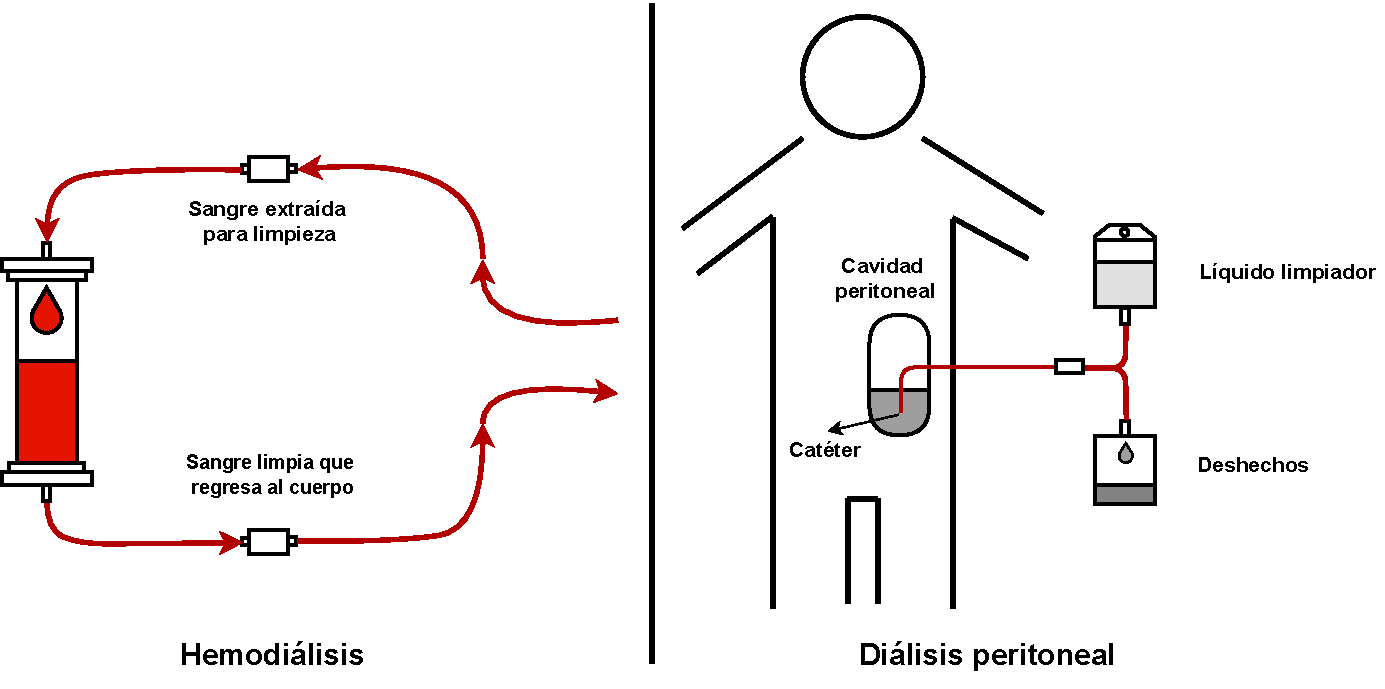
\includegraphics[width=.95\textwidth]{./Figures/Dialisis.pdf}
\caption{Diferencia entre hemodiálisis y diálisis peritoneal.}
\label{fig:diagDialisis}
\end{figure}


\section{Contexto y motivación}

La motivación principal de este trabajo es incorporar técnicas de inteligencia artificial (IA) en el campo de la medicina, dado que han demostrado una notable capacidad para anticipar eventos futuros basándose en datos históricos \citep{ARTICULO2}. 
Pero uno de los desafíos recurrentes a la hora de entrenar modelos de IA es la obtención de datos representativos. En el ámbito de la medicina este desafío también se hace presente, ya que se suele contar con pocos datos médicos de una población muy reducida.
Para el desarrollo de este trabajo se contó con datos médicos de unos catorce mi pacientes que estuvieron bajo tratamiento de diálisis renal. 
Tanto el equipo de sistemas como el equipo médico de ésta empresa de diálisis renal, si bien no tienen experiencias en herramientas de IA para predicción de eventos, conocen el potencial de estos modelos para identificar patrones, por lo que colaboraron en el desarrollo de este trabajo para lograr el cumplimiento del objetivo.

%----------------------------------------------------------------------------------------

\section{Objetivos, alcance y requerimientos}

\subsection{Objetivos}

El propósito de este trabajo fue el desarrollo de un modelo de IA que permite predecir el riesgo de mortalidad en pacientes en diálisis renal, junto con la configuración de una plataforma de administración de modelos, una interfaz de comunicación con el modelo y un proceso que solicite las predicciones continuamente. Este conjunto de herramientas provee una predicción actualizada del riego de mortalidad de los pacientes, lo que permite al personal médico adaptar el tratamiento y la medicación prescrita para mejorarles su calidad de vida y, en última instancia, salvar vidas. En la figura \ref{fig:diagArqBasic} se muestra la arquitectura de la solución propuesta. 

\begin{figure}[htpb]
\centering 
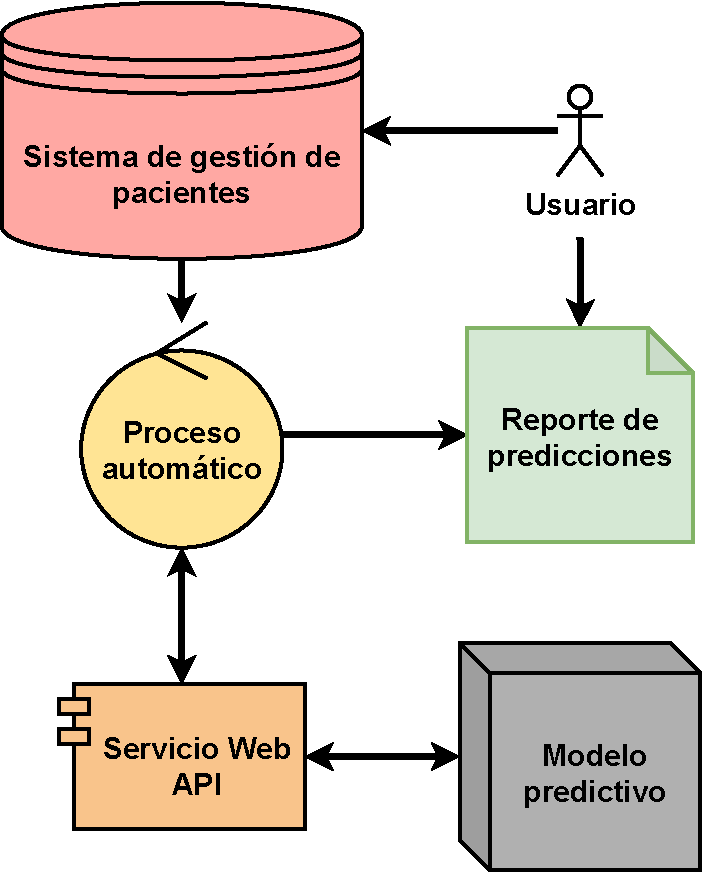
\includegraphics[width=.50\textwidth]{./Figures/Arquiectura_Solucion_Basica.pdf}
\caption{Arquitectura de solución.}
\label{fig:diagArqBasic}
\end{figure}


\subsection{Alcance}

Se encuentra dentro del alcance del trabajo la instalación y configuración de una plataforma de gestión de modelos que permite desplegar modelos en distintos ambientes, el desarrollo de un modelo de predicción de mortalidad, y la construcción de una interfaz y un proceso automático que actúan como nexo entre el modelo predictivo y el sistema de gestión de pacientes.
Para el desarrollo del modelo, se elabora un conjunto de datos con variables médicas de pacientes en diálisis renal. El conjunto de datos debe estar en cumplimiento con la ley 25.326 para garantizar el derecho al honor y a la intimidad de los pacientes en cuestión. Asimismo, se incluye en el alcance el pre-procesamiento del conjunto de datos y el análisis de las distintas métricas para evaluar el correcto desempeño del modelo.

Sin embargo, no se encuentra dentro del alcance del proyecto el desarrollo de una plataforma de gestión, sino que se eligió una existente que cumple con los requerimientos del trabajo, ni el desarrollo de una interfaz web orientada al usuario final. Tampoco se encuentra dentro del alcance la instalación del modelo predictivo en el entorno productivo de la empresa médica. Lo único que se instala en el entorno de la empresa médica será el proceso que recupera datos de los pacientes y llama al servicio web cada cierto período de tiempo para recuperar las predicciones. 

\subsection{Requerimientos}
A continuación, se listan los requerimientos principales del trabajo agrupados por afinidad:
\begin{enumerate}
	\item Requerimientos funcionales
		\begin{enumerate}
			\item La plataforma de gestión de modelos deberá permitir desplegar modelos en diversos ambientes.
			\item La interfaz por servicio web deberá recibir datos médicos de uno o varios pacientes y devolver las predicciones asociadas a ellos.			
			\item El modelo predictivo deberá tener una precisión de al menos un 75\%.
			\item El proceso que solicita predicciones y genera el reporte al usuario deberá poder ejecutarse automáticamente cada cierto período de tiempo.		
			\item El reporte de predicciones que le llegue al usuario final deberá tener un formato claro y comprensible.
			\item Se utilizará GIT como repositorio para el control de version de código
		\end{enumerate}
	\item Requerimientos de datos a utilizar
		\begin{enumerate}		
		\item Durante el entrenamiento del modelo se deberá resguardar la confidencialidad de los datos de los pacientes.		
		\end{enumerate}
	\item Requerimientos de documentación
		\begin{enumerate}
			\item Redactar una memoria técnica con la información del proyecto.
			\item La documentación de la interfaz por servicio web deberá incluir la lista de métodos disponibles con su detalle.
			\item La documentación del modelo predictivo incluirá información sobre el origen de los datos utilizados para el entrenamiento, las características que se usaron, el detalle del modelo seleccionado y la información que haya sobre la explicabilidad del modelo.
		\end{enumerate}		
\end{enumerate}

%----------------------------------------------------------------------------------------

\section{Estado del arte}

Se llevó a cabo una exhaustiva revisión de la literatura relacionada con la predicción de la mortalidad de pacientes en diálisis renal y se ha encontrado principalmente una tesis doctoral \citep{ARTICULO3} muy relevante que plantea un objetivo similar pero cuenta con muchos menos datos para el entrenamiento de los modelos. Si bien las variables médicas seleccionadas para realizar las predicciones en dicha tesis son muy similares a las que se seleccionaron en este trabajo, allí se plantea la discriminación de los casos según el tiempo que los pacientes llevan en diálisis, ya sea tres meses, seis meses, un año o más. Los modelos utilizados en dicha tesis incluyen Bósque Aleatorio (\textit{Random Forest}) y Regresión Logística, algunos de los cuales también fueron utilizados en este trabajo.
En cuanto a las conclusiones, para evaluar el desempeño de los modelos se utilizó la métrica de Área bajo la curva (AUC), la cual llega a valores entre 70\% y 73\%.
En esta tesis también se muestra qué variables tienen mas influencia al realizar la predicción de mortalidad del paciente, lo que resulta sumamente importante para el personal médico.
También se ha encontrado una investigación \citep{ARTICULO4} donde se utilizan técnicas de IA para predecir la mortalidad en pacientes con enfermedad renal crónica. La misma también cuenta con muy pocos datos de pacientes en diáfisis renal y, aunque no se da mucho detalle sobre el entrenamiento de los modelos, concluye indicando que con un modelo de red neuronal se obtiene una predicción superior al 90\%, mejor que con una Regresión Logística.
Por otro lado, se ha encontrado otra tesis \citep{ARTICULO5} orientada comprobar si el índice neutrófilo/linfocito es un predictor de mortalidad en pacientes que inician hemodiálisis. Si bien no se entrena ningún modelo de IA en la investigación, se concluye en que dicho índice no es un predictor de la mortalidad pero que la edad mayor a 60 años si representa un factor de riesgo. 
Existen muchos otros trabajos relacionados con la temática de la predicción de mortalidad en pacientes con enfermedades renales, donde algunos abordan el beneficio que aporta la IA en la detección y predicción de eventos en medicina \citep{ARTICULO6}\citep{ARTICULO7}\citep{ARTICULO9}, otros la predicción de mortalidad teniendo enfermedad renal junto con enfermedad coronaria \citep{ARTICULO10}, y otros la predicción de contraer algún cáncer renal \citep{ARTICULO8}.

Si bien existe literatura académica que aborda el tema de la predicción de mortalidad de pacientes en diálisis renal, la mayoría de los trabajos se centran en investigaciones de carácter teórico y experimental, y además parten de conjuntos de datos muy chicos, lo cual no permite a los modelos generalizar el conocimiento para poder realizar predicciones correctas. Este trabajo se destaca por su enfoque práctico, ya que se desarrolla una herramienta concreta que pueda ser implementada en una empresa médica dedicada a la diálisis renal. Se espera obtener predicciones en tiempo real para los pacientes en diálisis renal y en base a su riesgo de mortalidad adecuar el tratamiento y la medicación prescrita. Esta iniciativa ofrece una solución práctica y viable en el ámbito clínico, lo que contribuye a mejorar la atención y seguimiento de los pacientes.
\chapter{Introducción específica} % Main chapter title

\label{Chapter2}

%----------------------------------------------------------------------------------------
%	SECTION 1
%----------------------------------------------------------------------------------------
El objetivo de este capítulo es proporcionar una base teórica para comprender las herramientas y métodos utilizados en el desarrollo de este trabajo. En particular, se mencionarán las técnicas para el preprocesamiento de los datos, estrategias para el balanceo de clases, un repaso por los distintos modelos de inteligencia artificial y las métricas utilizadas para su evaluación. También se mencionarán conceptos básicos sobre plataformas de gestión de modelos de IA y servicios web.

\section{Tratamiento de los datos}

Una vez que se obtienen los datos para el entrenamiento de modelos de inteligencia artificial, es fundamental realizar un proceso de tratamiento de los datos para asegurar su calidad y adecuación para el análisis.
En primer lugar, la división de los datos en conjuntos de entrenamiento y prueba es una práctica común. Esto se hace para evaluar el rendimiento del modelo de manera efectiva, utilizando un conjunto de datos separado para el entrenamiento y otro para la evaluación, lo que ayuda a evitar el sobreajuste y a evaluar la capacidad de generalización del modelo.

Un punto clave en el tratamiento de datos es la corrección de valores inconsistentes o nulos. Esto implica identificar y corregir valores atípicos, faltantes o errores de entrada que podrían distorsionar el análisis y afectar la precisión del modelo. El valor faltante puede darse por diversas razones, como errores durante el ingreso manual de datos, mediciones incorrectas, fallas en el experimento, entre otras \citep{CAP2ARTICULO1}. Los valores faltantes son una realidad común en cualquier conjunto de datos y pueden tener un impacto significativo en el análisis y la interpretación de los resultados. Por lo tanto, es crucial entender las causas subyacentes y abordarlas adecuadamente durante el proceso de tratamiento de datos. Usualmente los datos faltantes se clasifican en los siguientes grupos: 
\begin{itemize}
\item Falta completamente al azar (MCAR): La probabilidad de que un registro tenga un valor faltante para un atributo no depende ni de los datos observados ni de los datos faltantes. Por ejemplo una muestra de laboratorio que se pierde.
\item Falta al azar (MAR): Indica que la probabilidad de que un registro tenga un valor faltante para un atributo podría depender de los datos observados, pero no del valor del dato faltante en sí mismo. Por ejemplo las personas con ingresos más altos pueden ser menos propensas a revelarlos en una encuesta, pero si la falta de respuesta es aleatoria dentro de las clases de ingresos, los datos de ingresos son faltantes al azar.
\item Falta no al azar (MNAR): Implica que la probabilidad de que un registro tenga un valor faltante para un atributo podría depender del valor del atributo mismo. Por ejemplo un sensor que no detecta temperaturas por debajo de cierto umbral, o personas que no completan los ingresos anuales en encuestas si superan cierto valor.
\end{itemize}

Para resolver el problema de los valores faltantes, existen diversos métodos de imputación de dichos valores. Estos son algunos de los más utilizados:
\begin{itemize}
\item Imputación por la media o mediana: Se remplazan los valores faltantes con la media o la mediana de la variable correspondiente. Esto es simple y rápido, pero puede introducir sesgos si la distribución de los datos es asimétrica o tiene valores atípicos.
\item Imputación por el valor más frecuente: Se remplazan los valores faltantes con el valor más común de la variable. Es útil para variables categóricas o variables con una distribución de frecuencia clara.
\item Imputación por regresión: Se utilizan modelos de regresión para predecir los valores faltantes a partir de las variables restantes. Esto puede ser más preciso que los métodos anteriores, pero puede ser computacionalmente intensivo y requiere asumir una relación lineal entre las variables.
\item Imputación por vecinos más cercanos (KNN): Los valores faltantes se estiman a partir de los valores de observaciones similares en el espacio de características. Este método puede ser efectivo en conjuntos de datos con estructuras de vecindario claras, pero puede ser sensible a la elección de la métrica de distancia y número de vecinos.
\item Imputación Múltiple por Ecuaciones Encadenadas (MICE): Se imputan los valores faltantes mediante la estimación secuencial de modelos predictivos, utilizando las variables restantes como predictores. Este método captura la incertidumbre asociada con la imputación de valores faltantes y puede proporcionar estimaciones más precisas.
\end{itemize}

Si los datos faltantes se consideran completamente aleatorios (MCAR), los métodos de imputación simples como la imputación por la media o mediana pueden ser apropiados. Cuando los datos faltantes son aleatorios (MAR), se pueden utilizar métodos más sofisticados como la imputación por regresión que utilizan información de otras variables observadas. Para datos no aleatorios (MNAR), la elección del método de imputación es más compleja y puede requerir técnicas específicas que modelen la relación entre los datos faltantes y los observados. Siempre es importante tener en cuenta las limitaciones y el contexto específico del conjunto de datos al tomar decisiones sobre el tratamiento de valores faltantes.

Otra de las técnicas que se pueden aplicar a los datos es la discretización, que es la conversión de variables continuas en variables discretas o categóricas. Esta técnica ayuda a que los modelos generen reglas mas breves y comprensibles, reduciendo la complejidad, y también es útil para aumentar la generalización y precisión del conocimiento \citep{CAP2ARTICULO2}.

Y por último, para obtener un conjunto de datos completamente numérico, se suele utilizar la codificación de variables categóricas. Esta técnica incluye métodos como la codificación \textit{one-hot} que convierte las variables categóricas en representaciones numéricas, asignando un valor binario a cada categoría. Además existen otras técnicas de codificación, como la codificación de etiquetas (\textit{label encoding}) y la codificación de frecuencia (\textit{frequency encoding}), que también se utilizan para transformar variables categóricas en datos numéricos compatibles con algoritmos de aprendizaje automático \citep{CAP2ARTICULO3}.

Las técnicas anteriormente mencionadas proveen soluciones a los problemas que suelen encontrarse en los conjuntos de datos y ayudan a garantizar la calidad y la adecuación para su posterior análisis y entrenamiento de modelos.


\section{Desbalance de clases}

El desbalance de clases es un problema común en el aprendizaje automático, donde una o más clases están subrepresentadas en comparación con otras en el conjunto de datos \citep{CAP2ARTICULO4}. Esto puede ser problemático porque los algoritmos de aprendizaje automático tienden a favorecer las clases mayoritarias y pueden tener dificultades para aprender patrones en las clases minoritarias.
El desbalance de clases puede llevar a modelos sesgados y poco precisos, especialmente en problemas de clasificación donde la precisión de las clases minoritarias es de particular interés, como la detección de fraudes, enfermedades o anomalías.

Algunas técnicas comunes para abordar el desbalance de clases incluyen:
\begin{itemize}
\item Submuestreo: Se reduce el número de muestras de las clases mayoritarias para equilibrar la proporción de clases. Esto puede ayudar a prevenir el sesgo hacia las clases mayoritarias, pero también puede resultar en la pérdida de información valiosa.
\item Sobremuestreo: Implica aumentar el número de muestras de las clases minoritarias mediante técnicas como la replicación de instancias o la generación de nuevas muestras sintéticas. Esto puede ayudar a mejorar la representación de las clases minoritarias y a evitar el sesgo hacia las clases mayoritarias.
\item Ponderación de clases: Algunos algoritmos de aprendizaje automático permiten asignar pesos diferentes a las clases para tener en cuenta el desbalance de clases durante el entrenamiento del modelo. Esto puede ayudar a compensar la falta de representación de las clases minoritarias.
\end{itemize}

En la figura \ref{fig:diagDesbalance} se muestra la diferencia entre las técnicas de submuestreo y sobremuestreo.

\begin{figure}[htpb]
\centering 
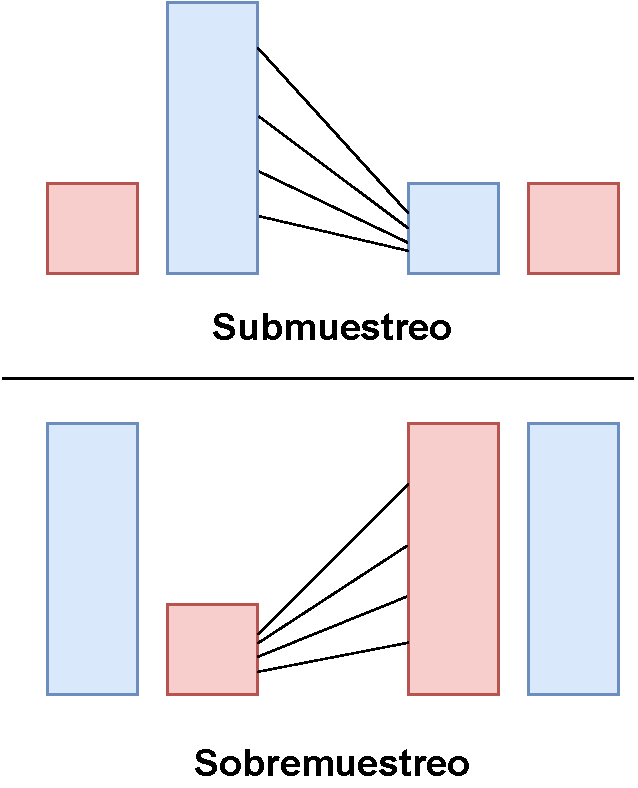
\includegraphics[width=.55\textwidth]{./Figures/Desbalance.pdf}
\caption{Submuestreo y sobremuestreo.}
\label{fig:diagDesbalance}
\end{figure}

Para el caso de submuestreo, existen varias técnicas utilizadas para equilibrar el desbalance de clases. Una de ellas es el submuestreo aleatorio (\textit{Random Undersampling}), donde se eliminan aleatoriamente un subconjunto de muestras de la clase mayoritaria para igualar el número de muestras de la clase minoritaria. Otra técnica es la de muestras cercanas (\textit{NearMiss}), que elimina muestras de la clase mayoritaria que están próximas a las muestras de la clase minoritaria en el espacio de características, preservando así la información relevante.

En cuanto al sobremuestreo, se puede aplicar la técnica de duplicación de muestras aleatorias (\textit{Random Oversampling}), que consiste en duplicar las muestras de la clase minoritaria para aumentar su representación en el conjunto de datos. Pero también existen técnicas para la generación de muestras sintéticas, como SMOTE (\textit{Synthetic Minority Over-sampling Technique}), que crea nuevas muestras interpoladas entre las muestras existentes de la clase minoritaria, lo que ayuda a mejorar su representación sin duplicar directamente las muestras existentes. 

Cada técnica tiene sus ventajas y desventajas y muchas veces se usa una combinación de ellas. La elección adecuada depende del conjunto de datos específico y del problema en cuestión. Es importante experimentar con diferentes enfoques y evaluar su rendimiento para determinar la estrategia más efectiva.


\section{Modelos de inteligencia artificial}

Los modelos de inteligencia artificial son comúnmente utilizados para reconocer patrones en grandes conjuntos de datos y obtener predicciones. Se dice que los modelos aprenden cuando logran mejorar sus resultados en una tarea específica luego de procesar muchos datos y sin obtener instrucciones explicitas de un programador \citep{ARTICULO2}. 
Los tipos de aprendizaje se dividen en los siguientes tres:
\begin{itemize}
\item Aprendizaje supervisado: Para entrenar al modelo se utiliza un conjunto de datos etiquetados. Esto quiere decir que se le provee tanto las características como el valor objetivo esperado. El modelo aprende a hacer predicciones basadas en estos ejemplos y se ajusta para minimizar los errores entre las predicciones y las etiquetas conocidas.
\item Aprendizaje no supervisado: No se utilizan etiquetas en los datos de entrenamiento. El modelo explora patrones y estructuras en los datos sin una guía explícita. Este enfoque es útil cuando no conocemos las categorías de antemano y queremos descubrir patrones ocultos.
\item Aprendizaje por refuerzo: El modelo aprende a tomar decisiones a través de la interacción con un entorno. Para cada acción recibirá recompensas o castigos según su desempeño. El objetivo es maximizar las recompensas a lo largo del tiempo.
\end{itemize}

Teniendo los datos y el tipo de aprendizaje que se desea implementar, se debe buscar también una arquitectura de modelo que tenga la capacidad de aprender de los datos y devolver predicciones. 
Dentro de la inteligencia artificial, existe un universo que se conoce como \textit{Machine Learning} (ML) o aprendizaje automático, que refiere a aquellos algoritmos que utilizan métodos estadísticos para analizar datos, aprender de ellos y elaborar predicciones o sugerencias. Entre los modelos de ML mas conocidos se encuentran los siguientes:

\begin{itemize}
\item Regresión Lineal: Se utiliza para predecir valores continuos basados en variables independientes. Busca la relación lineal entre las variables de entrada y salida.
\item Regresión Logística: Se utiliza para clasificación binaria. Estima la probabilidad de que una instancia pertenezca a una determinada clase.
\item Árboles de Decisión: Organizan las características de los datos en una estructura similar a un árbol. Cada nodo en este árbol representa una pregunta sobre una característica específica de los datos. Por ejemplo, podría ser ¿Tiene diabetes? o ¿Es menor de 30 años?. Las ramas del árbol representan las posibles respuestas a estas preguntas, como sí o no. Siguiendo las ramas del árbol, eventualmente se llega a una hoja que representa la decisión o predicción final.
\item Random Forest: Es una técnica de conjunto que combina múltiples árboles de decisión. Cada árbol se entrena con una muestra aleatoria del conjunto de datos y luego las predicciones se promedian para obtener la salida final.
\item Support Vector Machine (SVM): Es un algoritmo de clasificación que encuentra el hiperplano óptimo que mejor separa las clases en un espacio de características de alta dimensión. Puede ser usado tanto para clasificación como para regresión.
\end{itemize}

Dentro del universo ML, hay otro grupo mas chico que se denomina \textit{Deep Learning} (DL) o aprendizaje profundo, en donde los algoritmos utilizan una arquitectura de redes neuronales que simulan el comportamiento del cerebro humano, por lo que suelen ser mucho mas grandes y complejos.
Estos últimos suelen usarse para tareas de visión por computadora o procesamiento de lenguaje natural, y requieren mucha potencia de cómputo y grandes cantidades de datos.
En la figura \ref{fig:diagMLvsDL} se puede visualizar la diferencia entre utilizar modelos de \textit{Machine Learning} y modelos de \textit{Deep Learning} para obtener predicciones.

\begin{figure}[htpb]
\centering 
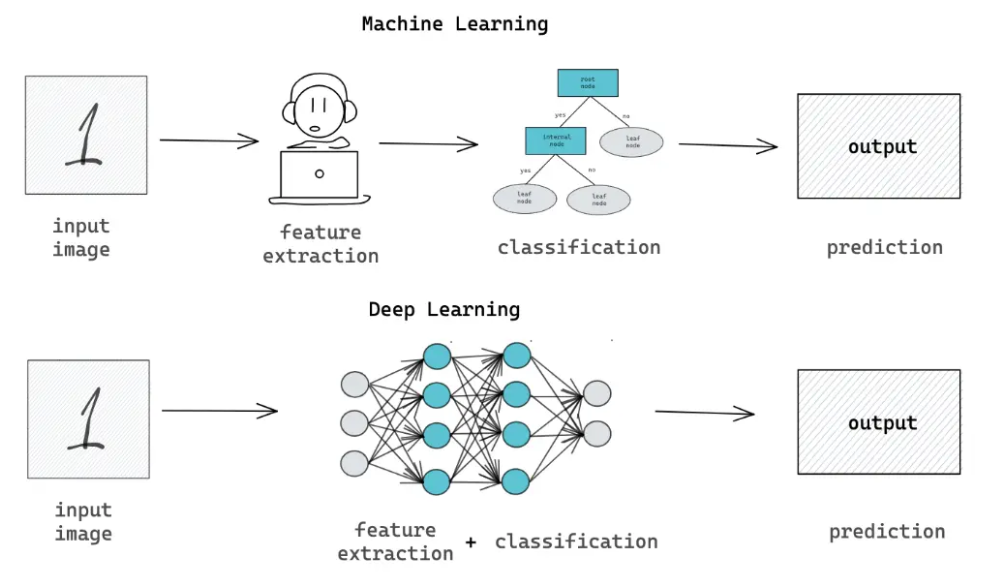
\includegraphics[width=.95\textwidth]{./Figures/ML vs DL.png}
\caption{Machine Learning vs Deep Learning.}
\label{fig:diagMLvsDL}
\end{figure}

Los modelos también se diferencian por el tipo de predicción que realizan. Un modelo que predice un valor continuo, como el precio de una vivienda, se lo conoce como modelo de regresión. Mientras que a un modelo que predice una etiqueta o clase, ya sea binaria o multi-clase, se lo conoce como modelo de clasificación. 

Este último tipo de modelo es muy utilizado en medicina, ya que sirve para predecir la presencia o ausencia de cierta enfermedad, o para predecir su tipo específico.
En este trabajo en particular, se utilizaron modelos de clasificación con aprendizaje supervisado. Se usaron arquitecturas de modelos de \textit{Machine Learning} y de \textit{Deep Learning} con el propósito de predecir el riesgo de mortalidad de pacientes en diálisis renal. Es importante señalar que se trata de una clasificación binaria puesto que la variable objetivo tiene dos posibles valores: no hay riesgo ("0") o hay riesgo ("1") de mortalidad.

\section{Evaluación de modelos de clasificación}

Para evaluar el comportamiento de un modelo de clasificación binaria comúnmente se recurre a una herramienta llamada matriz de confusión. Esta matriz, como se muestra en la figura \ref{fig:MatrizConfusion}, presenta las clases predichas en las columnas y las clases reales en las filas. A partir de esta tabla, se derivan cuatro métricas clave:

\begin{figure}[htpb]
\centering 
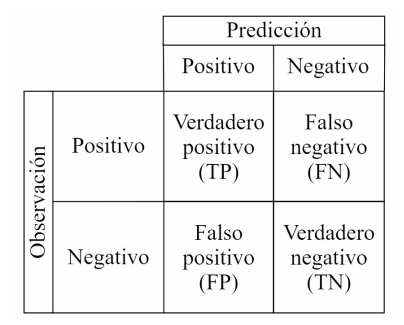
\includegraphics[width=.75\textwidth]{./Figures/MatrizDeConfusion.png}
\caption{Matriz de confusión.}
\label{fig:MatrizConfusion}
\end{figure}

\begin{itemize}
\item Verdaderos positivos (TP): Representan las predicciones correctas de una condición positiva.
\item Verdaderos negativos (TN): Son las predicciones correctas de una condición negativa.
\item Falsos positivos (FP): Se dan cuando el modelo predice incorrectamente una condición positiva que en realidad no lo es.
\item Falsos negativos (FN): Se dan cuando el modelo predice incorrectamente la ausencia de una condición positiva que en realidad está presente.
\end{itemize}

En contextos médicos, los falsos negativos pueden tener consecuencias significativas para la salud del paciente, ya que se está prediciendo que un paciente no tiene cierta condición cuando en realidad la tiene. 

Particularmente en este trabajo, los falsos negativos podrían implicar no tomar medidas necesarias para un tratamiento adecuado, aumentando el riesgo de mortalidad del paciente. Por lo tanto, es fundamental minimizar la tasa de falsos negativos tanto como sea posible, incluso si esto conlleva un aumento en los falsos positivos. 

Derivados de estos 4 valores de la matriz de confusión se definen las siguientes métricas para evaluar el rendimiento de un modelo de clasificación:

\begin{itemize}
\item \textit{Precision}: Es la proporción de ejemplos positivos que fueron correctamente clasificados como positivos respecto al total de ejemplos clasificados como positivos. Es decir, mide la calidad de las predicciones positivas del modelo. Se calcula como TP / (TP + FP).
\item \textit{Recall}: Es la proporción de ejemplos positivos que fueron correctamente clasificados como positivos respecto al total de ejemplos que son realmente positivos. Es decir, mide la capacidad del modelo para encontrar todos los ejemplos positivos. Se calcula como TP / (TP + FN).
\item \textit{F1 Score}: Es la media armónica de la \textit{precision} y el \textit{recall}. Proporciona un equilibrio entre ambas métricas y es útil cuando hay un desequilibrio entre las clases. Se calcula como 2 * (\textit{precision} * \textit{recall}) / (\textit{precision} + \textit{recall}).
\item \textit{Accuracy}: Es la proporción de ejemplos clasificados correctamente (tanto positivos como negativos) respecto al total de ejemplos. Es una métrica general de la calidad del modelo en todas las clases. Se calcula como (TP + TN) / (TP + TN + FP + FN).
\item AUC (\textit{Area Under the Curve}): El AUC es el área bajo la curva ROC (\textit{Receiver Operating Characteristic}). La curva ROC es una representación gráfica de la sensibilidad frente a la tasa de falsos positivos para diferentes umbrales de clasificación. El AUC mide la capacidad del modelo para distinguir entre clases positivas y negativas. Un valor de AUC cercano a 1 indica un buen rendimiento del modelo, mientras que un valor cercano a 0.5 indica un rendimiento aleatorio.
\end{itemize}

En este trabajo se utilizaron las métricas antes mencionadas para la evaluación de los modelos entrenados, prestando especial atención a las métricas de \textit{F1 Score} y \textit{Recall}, ya que existe un desbalance entre las clases y es importante detectar correctamente a la mayoría de casos positivos.

\section{Plataforma de gestión de modelos}

Una plataforma de gestión de modelos de IA es una herramienta diseñada para ayudar a los equipos de desarrollo y científicos de datos a gestionar, monitorear y desplegar modelos de manera eficiente. Estas plataformas ofrecen las siguientes ventajas:

\begin{itemize}
\item Centralización: Permiten centralizar todos los modelos en un único lugar, facilitando su gestión y acceso.
\item Implementación automatizada: Facilitan la implementación de modelos en entornos de producción, proporcionando herramientas para la integración continua y la implementación continua (CI/CD).
\item Versionado: Ofrecen capacidades de versionado para los modelos, lo que facilita el seguimiento de cambios y la colaboración entre equipos.
\end{itemize}

Existen múltiples plataformas para gestión de modelos \textit{Open Source}, tales como MLFlow, Apache Airflow o Jenkins, las cuales se conectan directamente con repositorios en la nube, como GitHub, y descargan modelos para aplicar en distintos ambientes. También cuentan con la posibilidad de realizar re-ntrenamientos automáticos de los modelos cuando se cuente con nuevos conjuntos de datos, aunque este punto queda fuera del alcance de este trabajo. En este trabajo se configura Jenkins como plataforma de gestión de modelos.

\section{Servicios Web}

Una vez que el modelo de IA fue entrenado y desplegado en un algún ambiente, el siguiente paso es exponerlo a través de un servicio web. Esto generalmente se logra mediante la creación de una API (\textit{Application Programming Interface}).
Comúnmente se utilizan APIs para la interacción entre diferentes sistemas informáticos, facilitando el intercambio de datos y la ejecución de funciones remotas. Se suele utilizar también para el desarrollo de aplicaciones web y móviles, para solicitar datos de alguna fuente de información como una base de datos.
Se caracterizan por estar estructurados con métodos que requieren parámetros específicos y proporcionan respuestas predefinidas, lo que simplifica la interacción entre sistemas. Esta estandarización les otorga independencia de plataforma y lenguaje, lo que los convierte en herramientas altamente adaptables y versátiles.

En esta caso, la API actúa como un intermediario entre la aplicación cliente y el modelo de IA, facilitando la comunicación y la interacción. Como primer paso, recibe los datos del cliente en un formato especificado y realiza el pre-procesamiento de los mismos, tal como se realizó durante el entrenamiento del modelo. Una vez procesados los datos se realiza la consulta al modelo de IA para obtener una predicción como respuesta. Dicha predicción es la que se devuelve al cliente como respuesta del llamado a la API.

En este trabajo se desarrolla una API para el acceso al modelo que contiene métodos para obtener predicciones individuales o masivas. También se desarrolla una aplicación cliente que llama automáticamente a la API cada cierto período de tiempo para solicitar predicciones y genera reportes para el usuario final. 
\include{Chapters/Chapter3}
\include{Chapters/Chapter4} 
\include{Chapters/Chapter5} 

%----------------------------------------------------------------------------------------
%	CONTENIDO DE LA MEMORIA  - APÉNDICES
%----------------------------------------------------------------------------------------

\appendix % indicativo para indicarle a LaTeX los siguientes "capítulos" son apéndices

% Incluir los apéndices de la memoria como archivos separadas desde la carpeta Appendices
% Descomentar las líneas a medida que se escriben los apéndices

%\include{Appendices/AppendixA}
%\include{Appendices/AppendixB}
%\include{Appendices/AppendixC}

%----------------------------------------------------------------------------------------
%	BIBLIOGRAPHY
%----------------------------------------------------------------------------------------

\Urlmuskip=0mu plus 1mu\relax
\raggedright
\printbibliography[heading=bibintoc]

%----------------------------------------------------------------------------------------

\end{document}  